\documentclass[a4paper]{article}

\usepackage{caption}
\usepackage{listings}
\usepackage{fancyhdr}
\usepackage[top=3cm,bottom=3cm,left=3cm,right=3cm]{geometry}
\usepackage{color}
\usepackage{amsmath}
\usepackage{graphicx}

\definecolor{dkgreen}{rgb}{0,0.6,0}
\definecolor{gray}{rgb}{0.5,0.5,0.5}
\definecolor{mauve}{rgb}{0.58,0,0.82}

\lstset{frame=tb,
  language=Octave,
  aboveskip=3mm,
  belowskip=3mm,
  showstringspaces=false,
  columns=flexible,
  basicstyle={\small\ttfamily},
  numbers=none,
  numberstyle=\tiny\color{gray},
  keywordstyle=\color{blue},
  commentstyle=\color{dkgreen},
  stringstyle=\color{mauve},
  breaklines=true,
  breakatwhitespace=true,
  tabsize=3
}

\newcommand{\HRule}{\rule{\linewidth}{0.5mm}}
\pagestyle{fancy}
\lfoot{\small \color{gray}Tom Peerdeman - 10266186}
\cfoot{\thepage}
\rfoot{\small \color{gray}Ren\'e Aparicio Sa\'ez - 10214054}
\lhead{\small \color{gray}Autonome Mobiele Robots}

\begin{document}
\begin{titlepage}
\begin{center}
\textsc{\Large Autonome Mobiele Robots}\\[0.5cm]
\HRule \\[0,4cm]
\textsc{\huge \bfseries NXT - lijn detectie met behulp van een omni-directionele camera}
\HRule \\[8cm]
\begin{minipage}{0.4\textwidth}
\begin{flushleft}\large
\emph{Auteurs: Tom Peerdeman \& Ren\'e Aparicio Saez}\\
\end{flushleft}
\end{minipage}
\begin{minipage}{0.4\textwidth}
\begin{flushright}\large
\emph{Datum: \today\\\hspace{1cm}}\\
\end{flushright}
\end{minipage}
\end{center}
\end{titlepage}

\section{Materiaal}
Om de experimenten uit dit rapport te kunnen uitvoeren zijn de volgende materialen gebruikt:\\
- PC/Laptop met Matlab\\
- Boek: Autonomous Mobile Robots 2th Edition - Roland Siegwart et al.\\
- NXT-Robot\\
- Logitech Webcam\\
- Gloeilamp\\
- Zwarte tape

\section{Introduction}
Een autonome mobiele robot moet kunnen bepalen waar hij wel of niet mag rijden. Het is daarom nodig om de robot sensoren te geven die hem vertellen waar hij wel en niet kan rijden. Met behulp van een omni-directionele camera en een lijn-detectie algoritme kan de robot bepalen waar hij wel en niet naartoe kan rijden. Met behulp van een gewone webcam en een bolling met een weerkaatsend oppervlak kan eenvoudig een omni-directioneel beeld gemaakt worden. De code voor het rechttrekken van het beeld en het detecteren van lijnen is meegeleverd. Er hoeft slechts bepaald te worden wat de parameters voor de code zijn.
\section{Methode}
Enkele fotos waren meegeleverd waarmee getest kon worden. Echter is besloten nieuwe fotos te maken. De robot moest nog worden aangepast. Door op de webcam een plastic buis met daarop gemonteerd een gloeilamp aan de robot vast te tapen is de omni-directionele camera gemaakt. In figuur \ref{fig:opstelling} is te zien hoe de gebruikte robot er uit zag. Aan de hand van de live beelden die de camera doorstuurde, konden enkel fotos gemaakt worden, waarmee verder gewerkt kon worden. De gemaakte fotos zijn van het formaat 'RGB24: 960 x 720'. De meegeleverde fotos waren van het kleinere formaat 'RGB24: 640 x 480'. Als de webcam met dit kleinere formaat opnames maakte, werd het beeld echter te wazig. Het grotere formaat behoudt de verhoudingen, en is scherper. Daarnaast zijn de opnames gemaakt met een verhoogd contrast. Dit zorgt ervoor dat er minder kleurverschil en minder ruis in het beeld aanwezig is.
\begin{figure}[h]
	\centering
	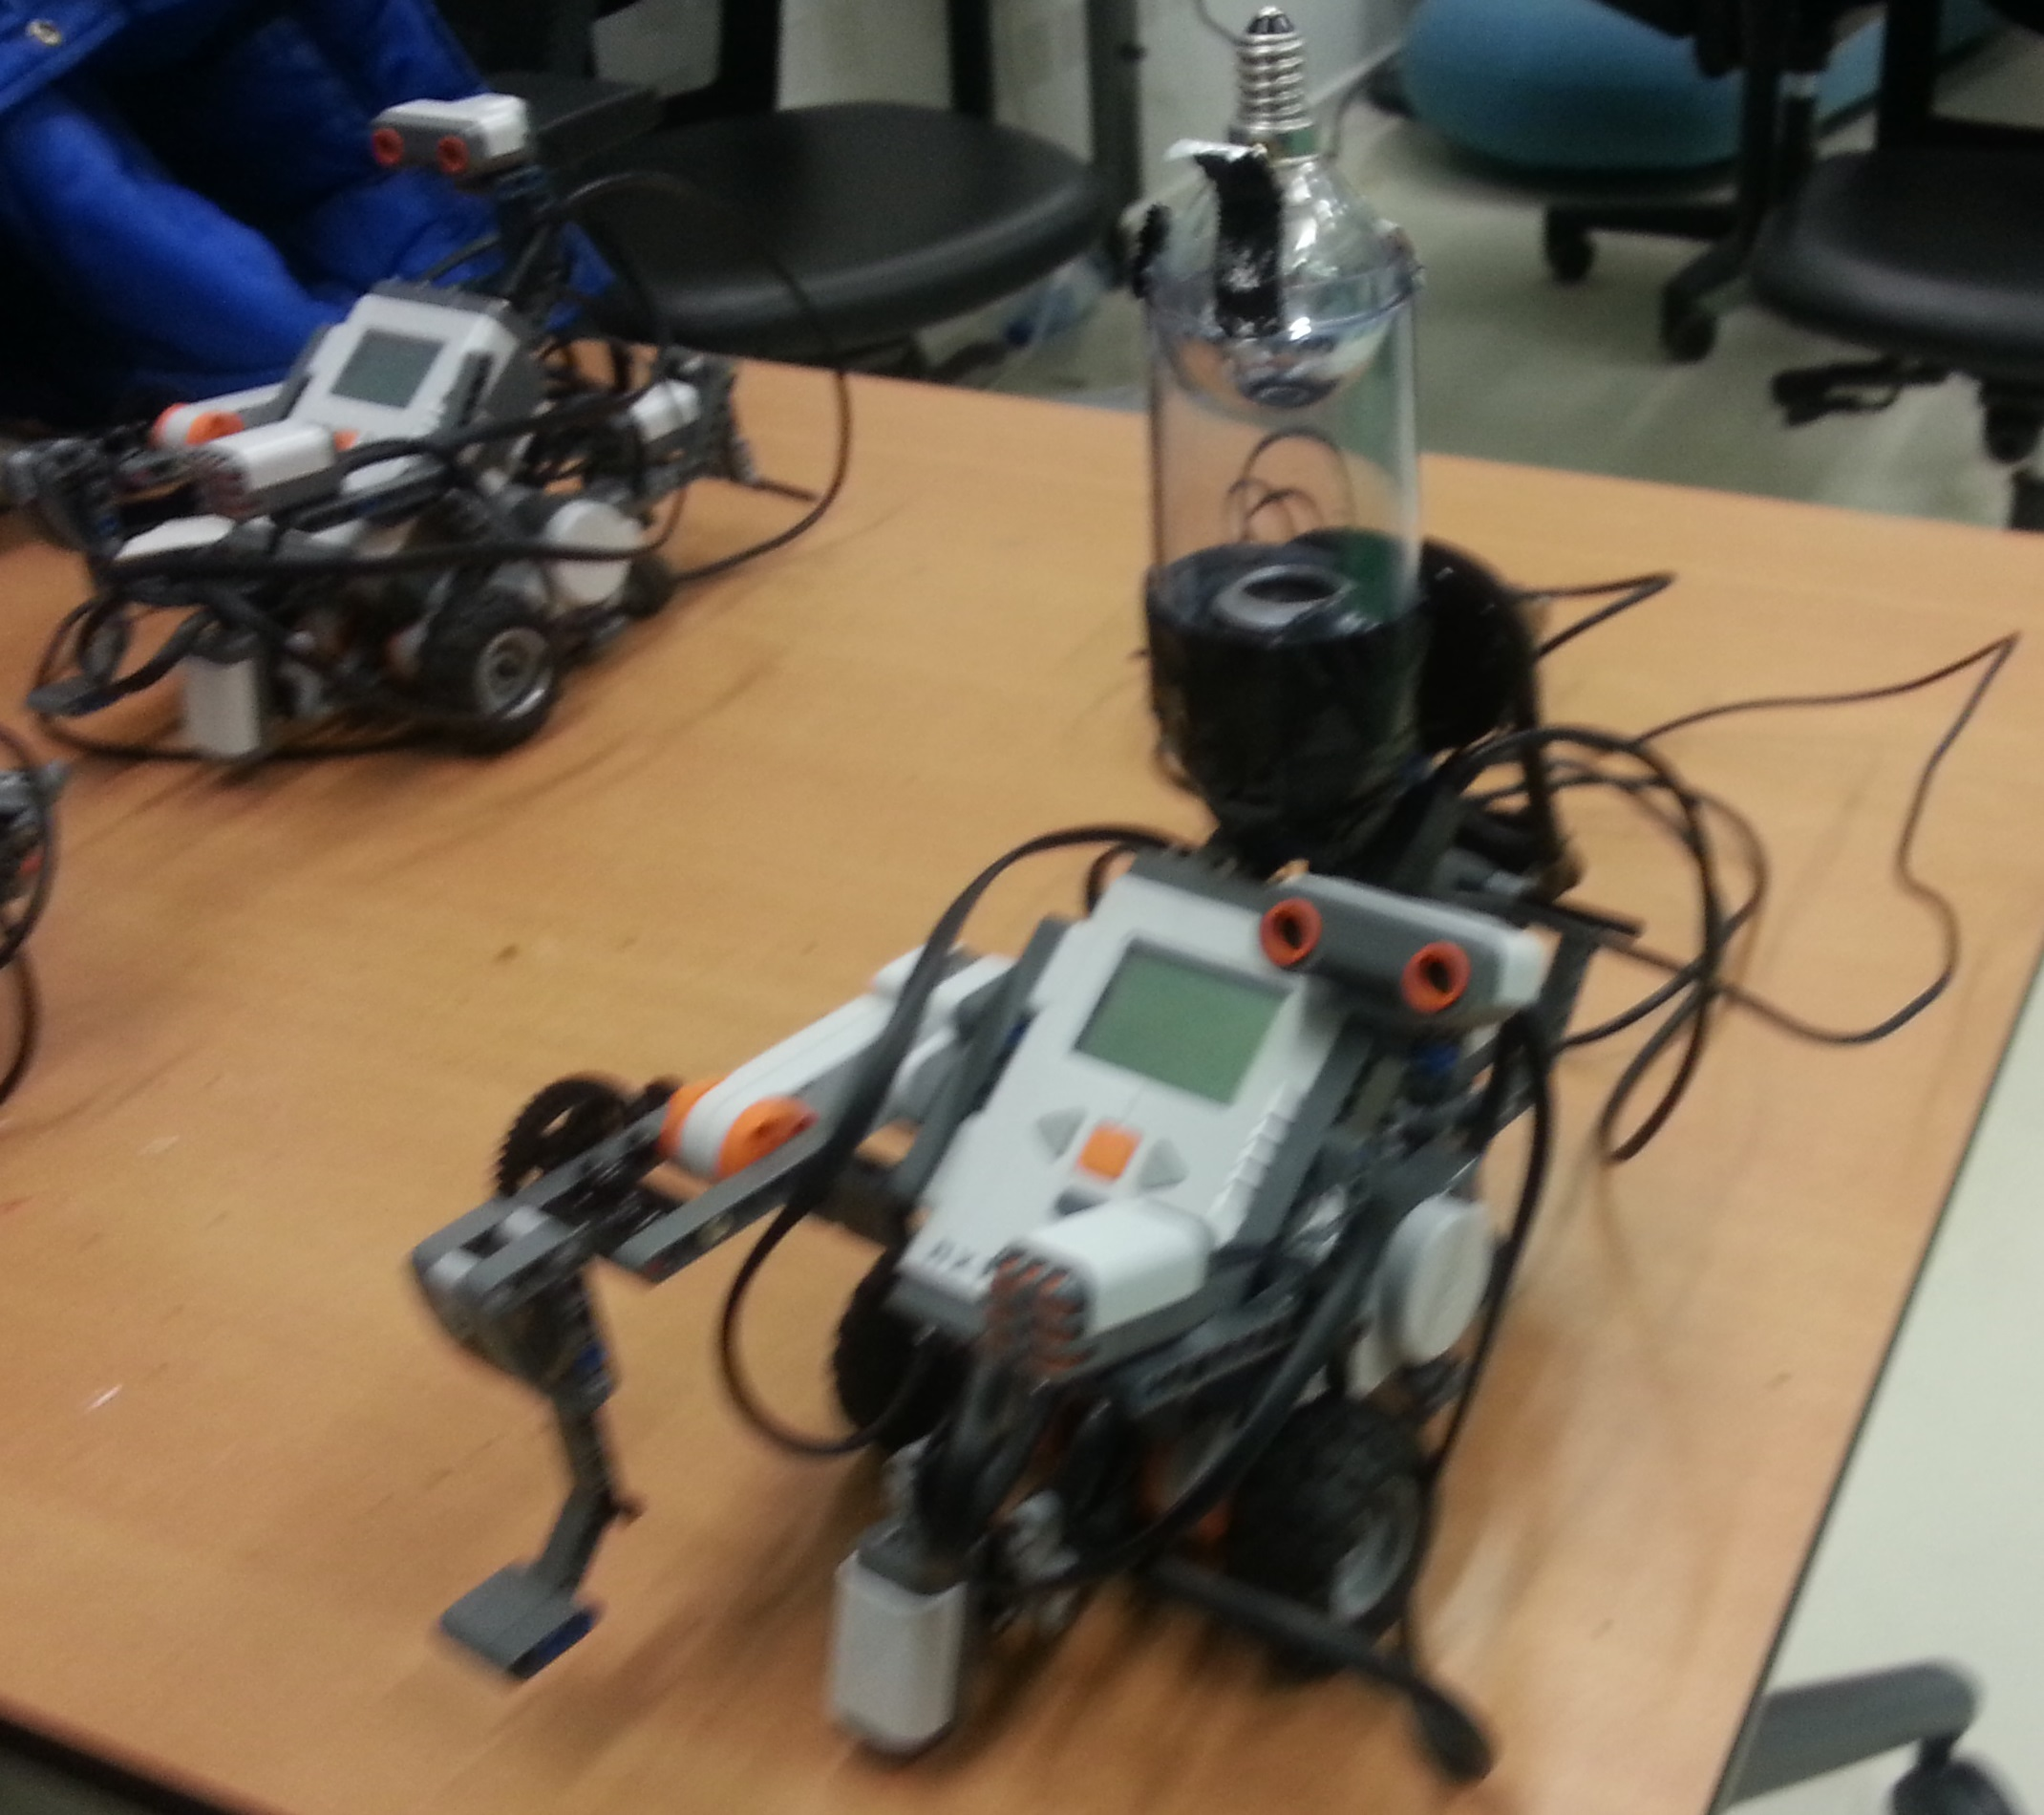
\includegraphics[width=0.7\textwidth]{img/opstelling.jpg}
	\caption{Originele robot links, aangepaste robot met camera rechts}
	\label{fig:opstelling}
\end{figure}
\section{Parameters bepalen}
\subsection{Calibreren van de camera}
De eerste parameters die moeten worden gekozen zijn de coordinaten voor het middelpunt van de camera. Zodra deze coordinaten zijn gevonden, kunnen deze in de code worden vastgelegd, omdat het middelpunt van de camera nooit zal veranderen (hierbij wordt er van uitgegaan dat de camera goed op de robot is gemonteerd en niet beweegt). Als het middelpunt van de camera goed is gekozen zal het uitgeklapte beeld, de rand van de camera in een rechte lijn plaatsen (zie figuur \ref{fig:incorrectcenter} en figuur \ref{fig:correctcenter}. Als dit niet het geval is zal de rand een slinger vertonen. Het middelpunt van de camera licht in het midden van de webcam, op de coordinaten $x = 444.2568$ en $y =333.2305$. Daarnaast moet de radius van de blinde vlek (de vlek waar de camera zichzelf ziet) worden bepaald. De radius van dit beeld is $radius = 90.4013$.
\begin{figure}[htbp]
  \begin{minipage}[b]{0.5\linewidth}
    \centering
    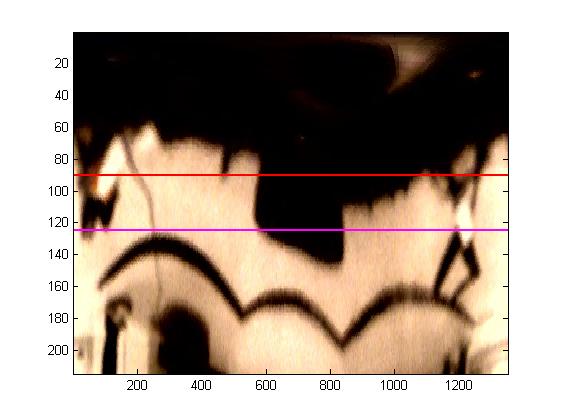
\includegraphics[width=\linewidth]{img/incorrect_center.png}
    \caption{Incorrect middelpunt}
    \label{fig:incorrectcenter}
  \end{minipage}
  \hspace{0.5cm}
  \begin{minipage}[b]{0.5\linewidth}
    \centering
    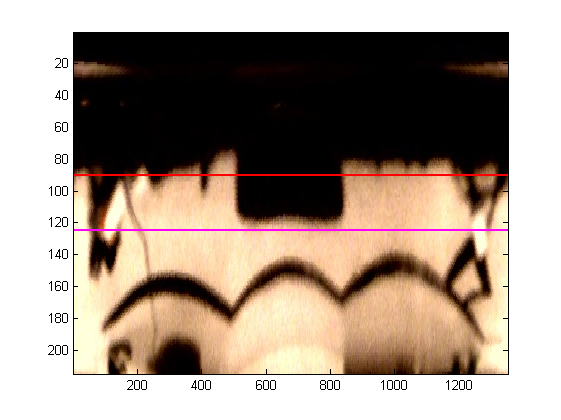
\includegraphics[width=\linewidth]{img/correct_center.png}
    \caption{Correct middelpunt}
    \label{fig:correctcenter}
  \end{minipage}
\end{figure}
\\
Bij het calibreren van de camera moet ook aangegeven worden naar welke afstanden gekeken moet worden, wordt er te dichtbij het midden van de webcam gezocht, zal de robot zichzelf zien en zal dit ruis gaan vormen. Kijkt de camera te ver door dan zal het beeld buiten de bolling vallen of te vere weg zijn om nog een goed resultaat op te leveren. De sensoren die aan de robot hangen steken helaas ver uit, dus moet er begonnen worden met kijken op een redelijk grote afstand bij de robot vandaan, $Rmin = 125$. De afstand tot waar gekeken mag worden kan vrij gekozen worden, zolang deze maar niet te ver weg ligt, $Rmax = 215$ . De waarden van de coordinaten, de radius, Rmin en Rmax zijn in pixels.
\subsection{Black-White Treshold}
Als de camera is gecalibreerd kan het beeld dat van belang is (het beeld tussen Rmin en Rmax) uit elkaar worden getrokken. Dit beeld wordt vervolgens omgezet in een zwart wit beeld aan de hand van een meegegeven treshold. Uit dit beeld kunnen vervolgens de lijnen worden gevonden die het dichtste bij de robot in de buurt liggen. Als de treshold niet goed wordt gekozen, zal het algoritme niet de volledige lijn vinden. Er moet dus een treshold worden gekozen die voldoende ruis wegfilterd, maar die wel de echte lijnen intact laat. In figuur zijn de resultaten voor verschillende tresholds te zien. Een treshold van 100 levert het beste resultaat op.
\begin{figure}[htbp]
  \begin{minipage}[b]{0.5\linewidth}
    \centering
    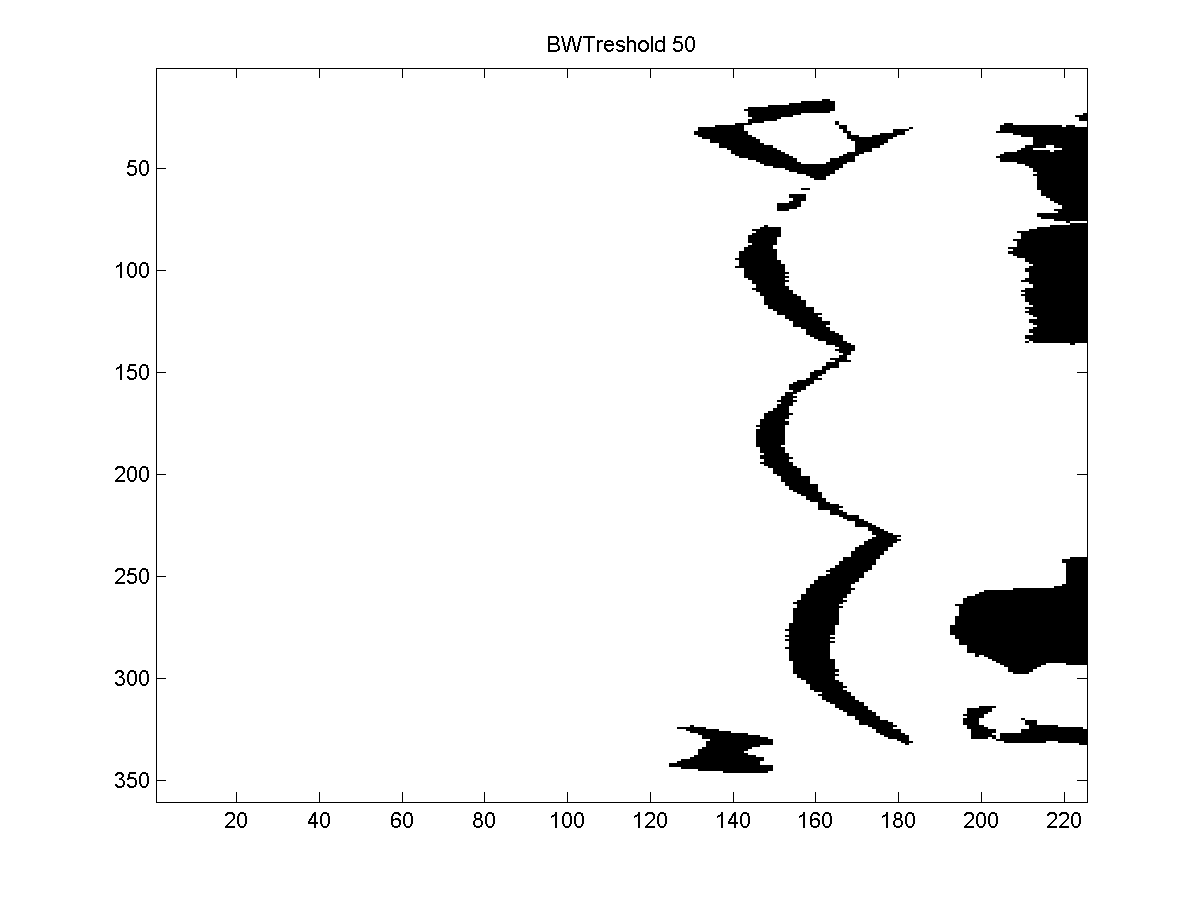
\includegraphics[width=\linewidth]{img/BWTreshold_50.png}
    \caption{Treshold = 50}
    \label{fig:bw50}
  \end{minipage}
  \hspace{0.5cm}
  \begin{minipage}[b]{0.5\linewidth}
    \centering
    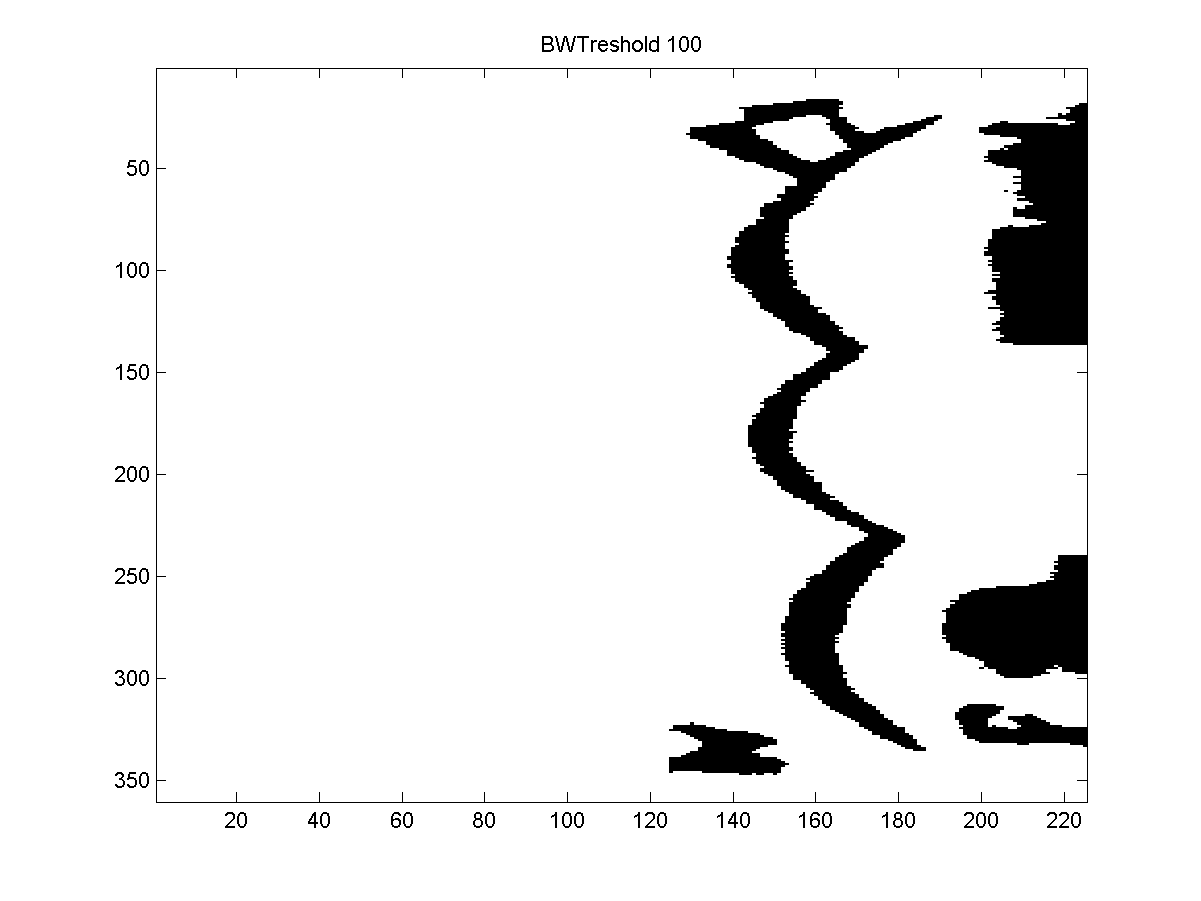
\includegraphics[width=\linewidth]{img/BWTreshold_100.png}
    \caption{Treshold = 100}
    \label{fig:bw100}
  \end{minipage}
\end{figure}
\begin{figure}[htbp]
  \begin{minipage}[b]{0.5\linewidth}
    \centering
    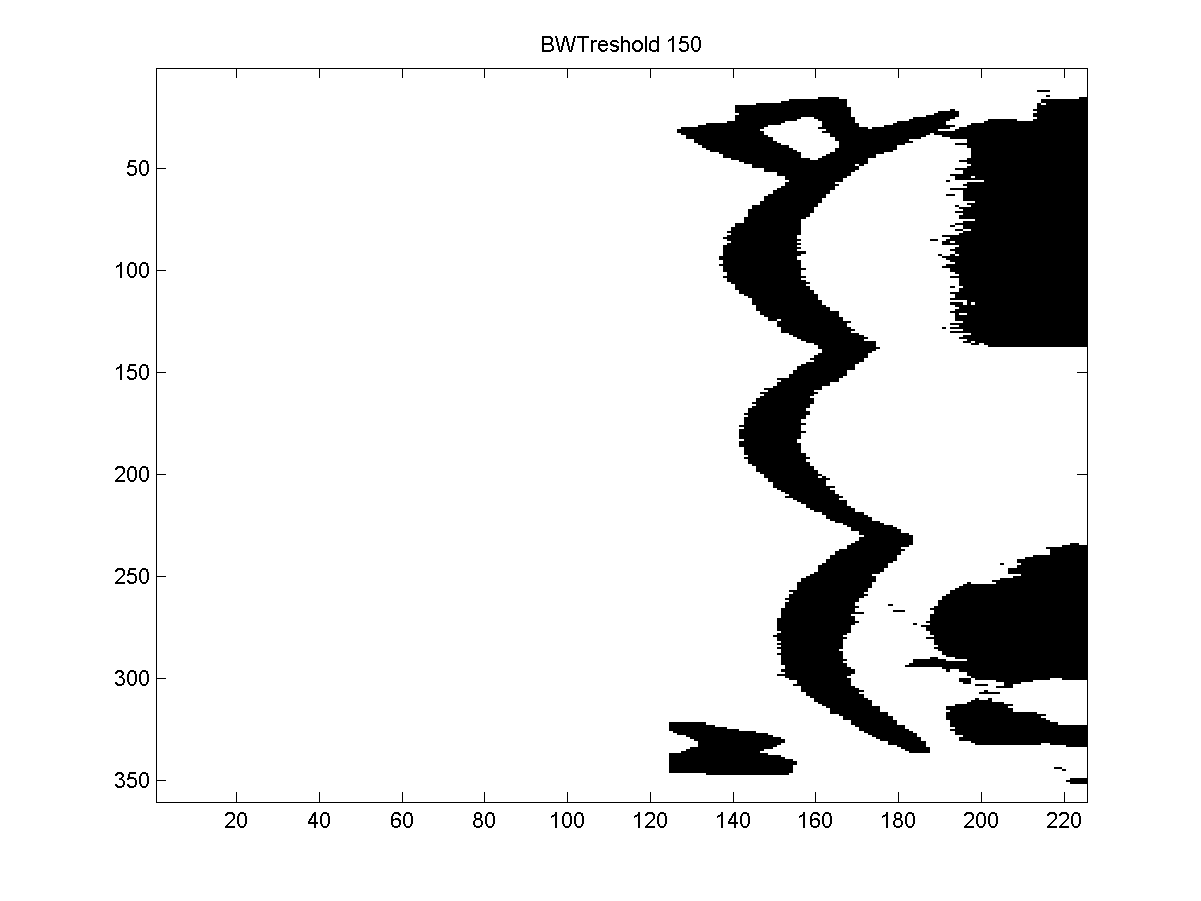
\includegraphics[width=\linewidth]{img/BWTreshold_150.png}
    \caption{Treshold = 150}
    \label{fig:bw150}
  \end{minipage}
  \hspace{0.5cm}
  \begin{minipage}[b]{0.5\linewidth}
    \centering
    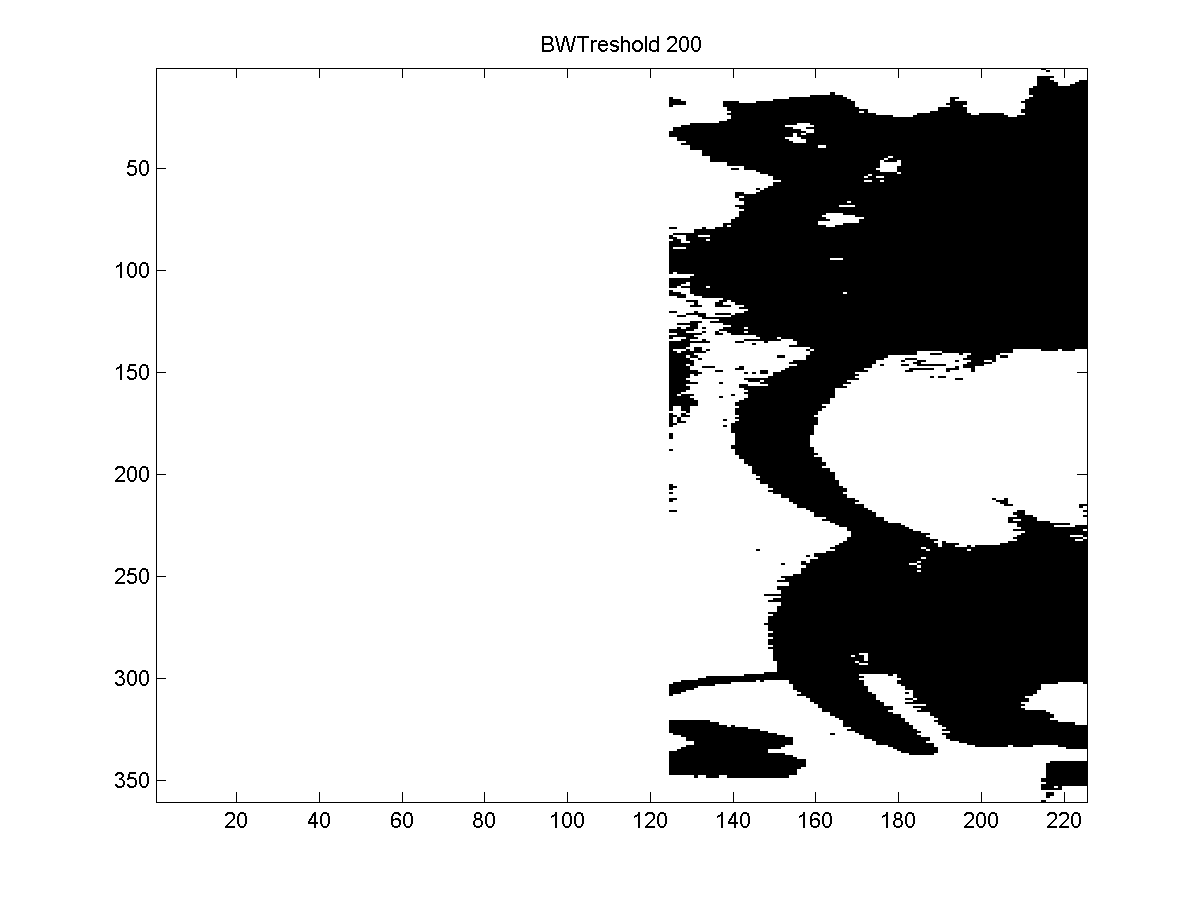
\includegraphics[width=\linewidth]{img/BWTreshold_200.png}
    \caption{Treshold = 200}
    \label{fig:bw200}
  \end{minipage}
\end{figure}
\section{Werkelijke afstand}
Als alle parameters zijn gevonden, kan uit het zwart wit beeld een lijst met pixelafstanden waorden opgemaakt tot de dichtsbijzijnde lijn. Echter Is het voor de gebruiker veel fijner om de afstanden in meters terug te krijgen. Aan de hand van de bolling, de hoogte van deze bolling ten opzichte van de camera en een gemeten werkelijke afstand kan een formule worden opgesteld die de pixelafstanden om kan zetten in werkelijke afstanden. 
\end{document}